% Options for packages loaded elsewhere
% Options for packages loaded elsewhere
\PassOptionsToPackage{unicode}{hyperref}
\PassOptionsToPackage{hyphens}{url}
\PassOptionsToPackage{dvipsnames,svgnames,x11names}{xcolor}
%
\documentclass[
  letterpaper,
  DIV=11,
  numbers=noendperiod]{scrartcl}
\usepackage{xcolor}
\usepackage[margin=1in]{geometry}
\usepackage{amsmath,amssymb}
\setcounter{secnumdepth}{-\maxdimen} % remove section numbering
\usepackage{iftex}
\ifPDFTeX
  \usepackage[T1]{fontenc}
  \usepackage[utf8]{inputenc}
  \usepackage{textcomp} % provide euro and other symbols
\else % if luatex or xetex
  \usepackage{unicode-math} % this also loads fontspec
  \defaultfontfeatures{Scale=MatchLowercase}
  \defaultfontfeatures[\rmfamily]{Ligatures=TeX,Scale=1}
\fi
\usepackage{lmodern}
\ifPDFTeX\else
  % xetex/luatex font selection
\fi
% Use upquote if available, for straight quotes in verbatim environments
\IfFileExists{upquote.sty}{\usepackage{upquote}}{}
\IfFileExists{microtype.sty}{% use microtype if available
  \usepackage[]{microtype}
  \UseMicrotypeSet[protrusion]{basicmath} % disable protrusion for tt fonts
}{}
\makeatletter
\@ifundefined{KOMAClassName}{% if non-KOMA class
  \IfFileExists{parskip.sty}{%
    \usepackage{parskip}
  }{% else
    \setlength{\parindent}{0pt}
    \setlength{\parskip}{6pt plus 2pt minus 1pt}}
}{% if KOMA class
  \KOMAoptions{parskip=half}}
\makeatother
% Make \paragraph and \subparagraph free-standing
\makeatletter
\ifx\paragraph\undefined\else
  \let\oldparagraph\paragraph
  \renewcommand{\paragraph}{
    \@ifstar
      \xxxParagraphStar
      \xxxParagraphNoStar
  }
  \newcommand{\xxxParagraphStar}[1]{\oldparagraph*{#1}\mbox{}}
  \newcommand{\xxxParagraphNoStar}[1]{\oldparagraph{#1}\mbox{}}
\fi
\ifx\subparagraph\undefined\else
  \let\oldsubparagraph\subparagraph
  \renewcommand{\subparagraph}{
    \@ifstar
      \xxxSubParagraphStar
      \xxxSubParagraphNoStar
  }
  \newcommand{\xxxSubParagraphStar}[1]{\oldsubparagraph*{#1}\mbox{}}
  \newcommand{\xxxSubParagraphNoStar}[1]{\oldsubparagraph{#1}\mbox{}}
\fi
\makeatother


\usepackage{longtable,booktabs,array}
\usepackage{calc} % for calculating minipage widths
% Correct order of tables after \paragraph or \subparagraph
\usepackage{etoolbox}
\makeatletter
\patchcmd\longtable{\par}{\if@noskipsec\mbox{}\fi\par}{}{}
\makeatother
% Allow footnotes in longtable head/foot
\IfFileExists{footnotehyper.sty}{\usepackage{footnotehyper}}{\usepackage{footnote}}
\makesavenoteenv{longtable}
\usepackage{graphicx}
\makeatletter
\newsavebox\pandoc@box
\newcommand*\pandocbounded[1]{% scales image to fit in text height/width
  \sbox\pandoc@box{#1}%
  \Gscale@div\@tempa{\textheight}{\dimexpr\ht\pandoc@box+\dp\pandoc@box\relax}%
  \Gscale@div\@tempb{\linewidth}{\wd\pandoc@box}%
  \ifdim\@tempb\p@<\@tempa\p@\let\@tempa\@tempb\fi% select the smaller of both
  \ifdim\@tempa\p@<\p@\scalebox{\@tempa}{\usebox\pandoc@box}%
  \else\usebox{\pandoc@box}%
  \fi%
}
% Set default figure placement to htbp
\def\fps@figure{htbp}
\makeatother





\setlength{\emergencystretch}{3em} % prevent overfull lines

\providecommand{\tightlist}{%
  \setlength{\itemsep}{0pt}\setlength{\parskip}{0pt}}



 


\KOMAoption{captions}{tableheading}
\makeatletter
\@ifpackageloaded{tcolorbox}{}{\usepackage[skins,breakable]{tcolorbox}}
\@ifpackageloaded{fontawesome5}{}{\usepackage{fontawesome5}}
\definecolor{quarto-callout-color}{HTML}{909090}
\definecolor{quarto-callout-note-color}{HTML}{0758E5}
\definecolor{quarto-callout-important-color}{HTML}{CC1914}
\definecolor{quarto-callout-warning-color}{HTML}{EB9113}
\definecolor{quarto-callout-tip-color}{HTML}{00A047}
\definecolor{quarto-callout-caution-color}{HTML}{FC5300}
\definecolor{quarto-callout-color-frame}{HTML}{acacac}
\definecolor{quarto-callout-note-color-frame}{HTML}{4582ec}
\definecolor{quarto-callout-important-color-frame}{HTML}{d9534f}
\definecolor{quarto-callout-warning-color-frame}{HTML}{f0ad4e}
\definecolor{quarto-callout-tip-color-frame}{HTML}{02b875}
\definecolor{quarto-callout-caution-color-frame}{HTML}{fd7e14}
\makeatother
\makeatletter
\@ifpackageloaded{caption}{}{\usepackage{caption}}
\AtBeginDocument{%
\ifdefined\contentsname
  \renewcommand*\contentsname{Table of contents}
\else
  \newcommand\contentsname{Table of contents}
\fi
\ifdefined\listfigurename
  \renewcommand*\listfigurename{List of Figures}
\else
  \newcommand\listfigurename{List of Figures}
\fi
\ifdefined\listtablename
  \renewcommand*\listtablename{List of Tables}
\else
  \newcommand\listtablename{List of Tables}
\fi
\ifdefined\figurename
  \renewcommand*\figurename{Figure}
\else
  \newcommand\figurename{Figure}
\fi
\ifdefined\tablename
  \renewcommand*\tablename{Table}
\else
  \newcommand\tablename{Table}
\fi
}
\@ifpackageloaded{float}{}{\usepackage{float}}
\floatstyle{ruled}
\@ifundefined{c@chapter}{\newfloat{codelisting}{h}{lop}}{\newfloat{codelisting}{h}{lop}[chapter]}
\floatname{codelisting}{Listing}
\newcommand*\listoflistings{\listof{codelisting}{List of Listings}}
\makeatother
\makeatletter
\makeatother
\makeatletter
\@ifpackageloaded{caption}{}{\usepackage{caption}}
\@ifpackageloaded{subcaption}{}{\usepackage{subcaption}}
\makeatother
\usepackage{bookmark}
\IfFileExists{xurl.sty}{\usepackage{xurl}}{} % add URL line breaks if available
\urlstyle{same}
\hypersetup{
  pdftitle={Chromosomes},
  colorlinks=true,
  linkcolor={blue},
  filecolor={Maroon},
  citecolor={Blue},
  urlcolor={Blue},
  pdfcreator={LaTeX via pandoc}}


\title{Chromosomes}
\author{}
\date{}
\begin{document}
\maketitle

\renewcommand*\contentsname{Table of contents}
{
\hypersetup{linkcolor=}
\setcounter{tocdepth}{3}
\tableofcontents
}

\subsection{Why chromosomes matter}\label{why-chromosomes-matter}

\begin{itemize}
\tightlist
\item
  what a \textbf{chromosome} is
\item
  how chromosomes differ from each other
\item
  what it means for chromosomes to be \textbf{homologous}
\end{itemize}

This section builds the mental model you'll use all semester.

\begin{center}\rule{0.5\linewidth}{0.5pt}\end{center}

\subsection{What is a chromosome?}\label{what-is-a-chromosome}

A \textbf{chromosome} is: - one single DNA molecule - packaged with
proteins - containing many genes and many sections without genes
(intergenic regions) - defined by the genes it carries

\begin{tcolorbox}[enhanced jigsaw, colframe=quarto-callout-important-color-frame, leftrule=.75mm, bottomrule=.15mm, opacitybacktitle=0.6, opacityback=0, left=2mm, rightrule=.15mm, coltitle=black, bottomtitle=1mm, titlerule=0mm, toptitle=1mm, breakable, title=\textcolor{quarto-callout-important-color}{\faExclamation}\hspace{0.5em}{Key idea}, colbacktitle=quarto-callout-important-color!10!white, arc=.35mm, toprule=.15mm, colback=white]

A chromosome is not a single gene --- it is a \textbf{collection of many
genes and intergenic regions arranged along one DNA molecule}.

\end{tcolorbox}

\subsection{Chromosomes can be different
shapes}\label{chromosomes-can-be-different-shapes}

\begin{itemize}
\tightlist
\item
  Some chromosomes are linear (like a piece of spagetti)
\item
  Some chromosomes are circular (like a fruit loop)
  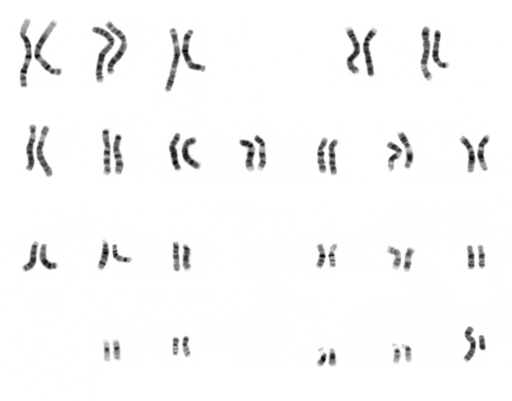
\includegraphics[width=0.5\linewidth,height=\textheight,keepaspectratio]{../images/human_male_karyotype.png}
  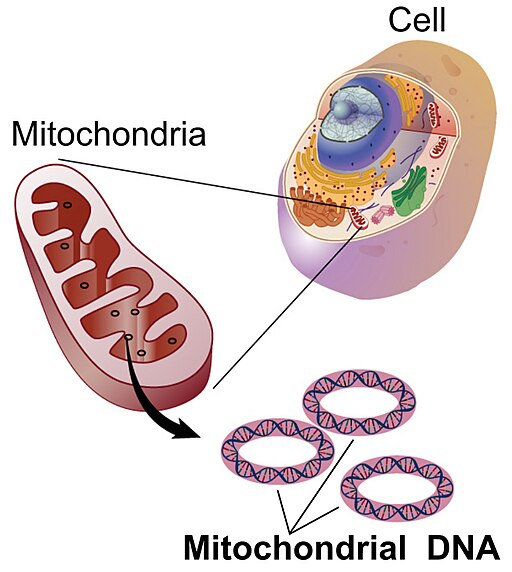
\includegraphics[width=0.5\linewidth,height=\textheight,keepaspectratio]{../images/mitochondria.png}
  \emph{Figure 1. A human male karyotype showing linear chromosomes.}
  Image source: National Human Genome Research Institute, Public domain,
  via Wikimedia Commons. \emph{Figure 2. A cell, mitochondria, and
  representation of mitochondrial circular DNA} Image Source: Science
  Primer (National Center for Biotechnology Information). Vectorized by
  Mortadelo2005., Public domain, via Wikimedia Commons
\end{itemize}

\begin{center}\rule{0.5\linewidth}{0.5pt}\end{center}

\subsection{Different chromosomes carry different
genes}\label{different-chromosomes-carry-different-genes}

Each chromosome type carries a \textbf{different set of genes}.

\textbf{What to notice} - Chromosome 1 has genes that chromosome 2 does
not - Chromosome 2 has genes that chromosome 3 does not

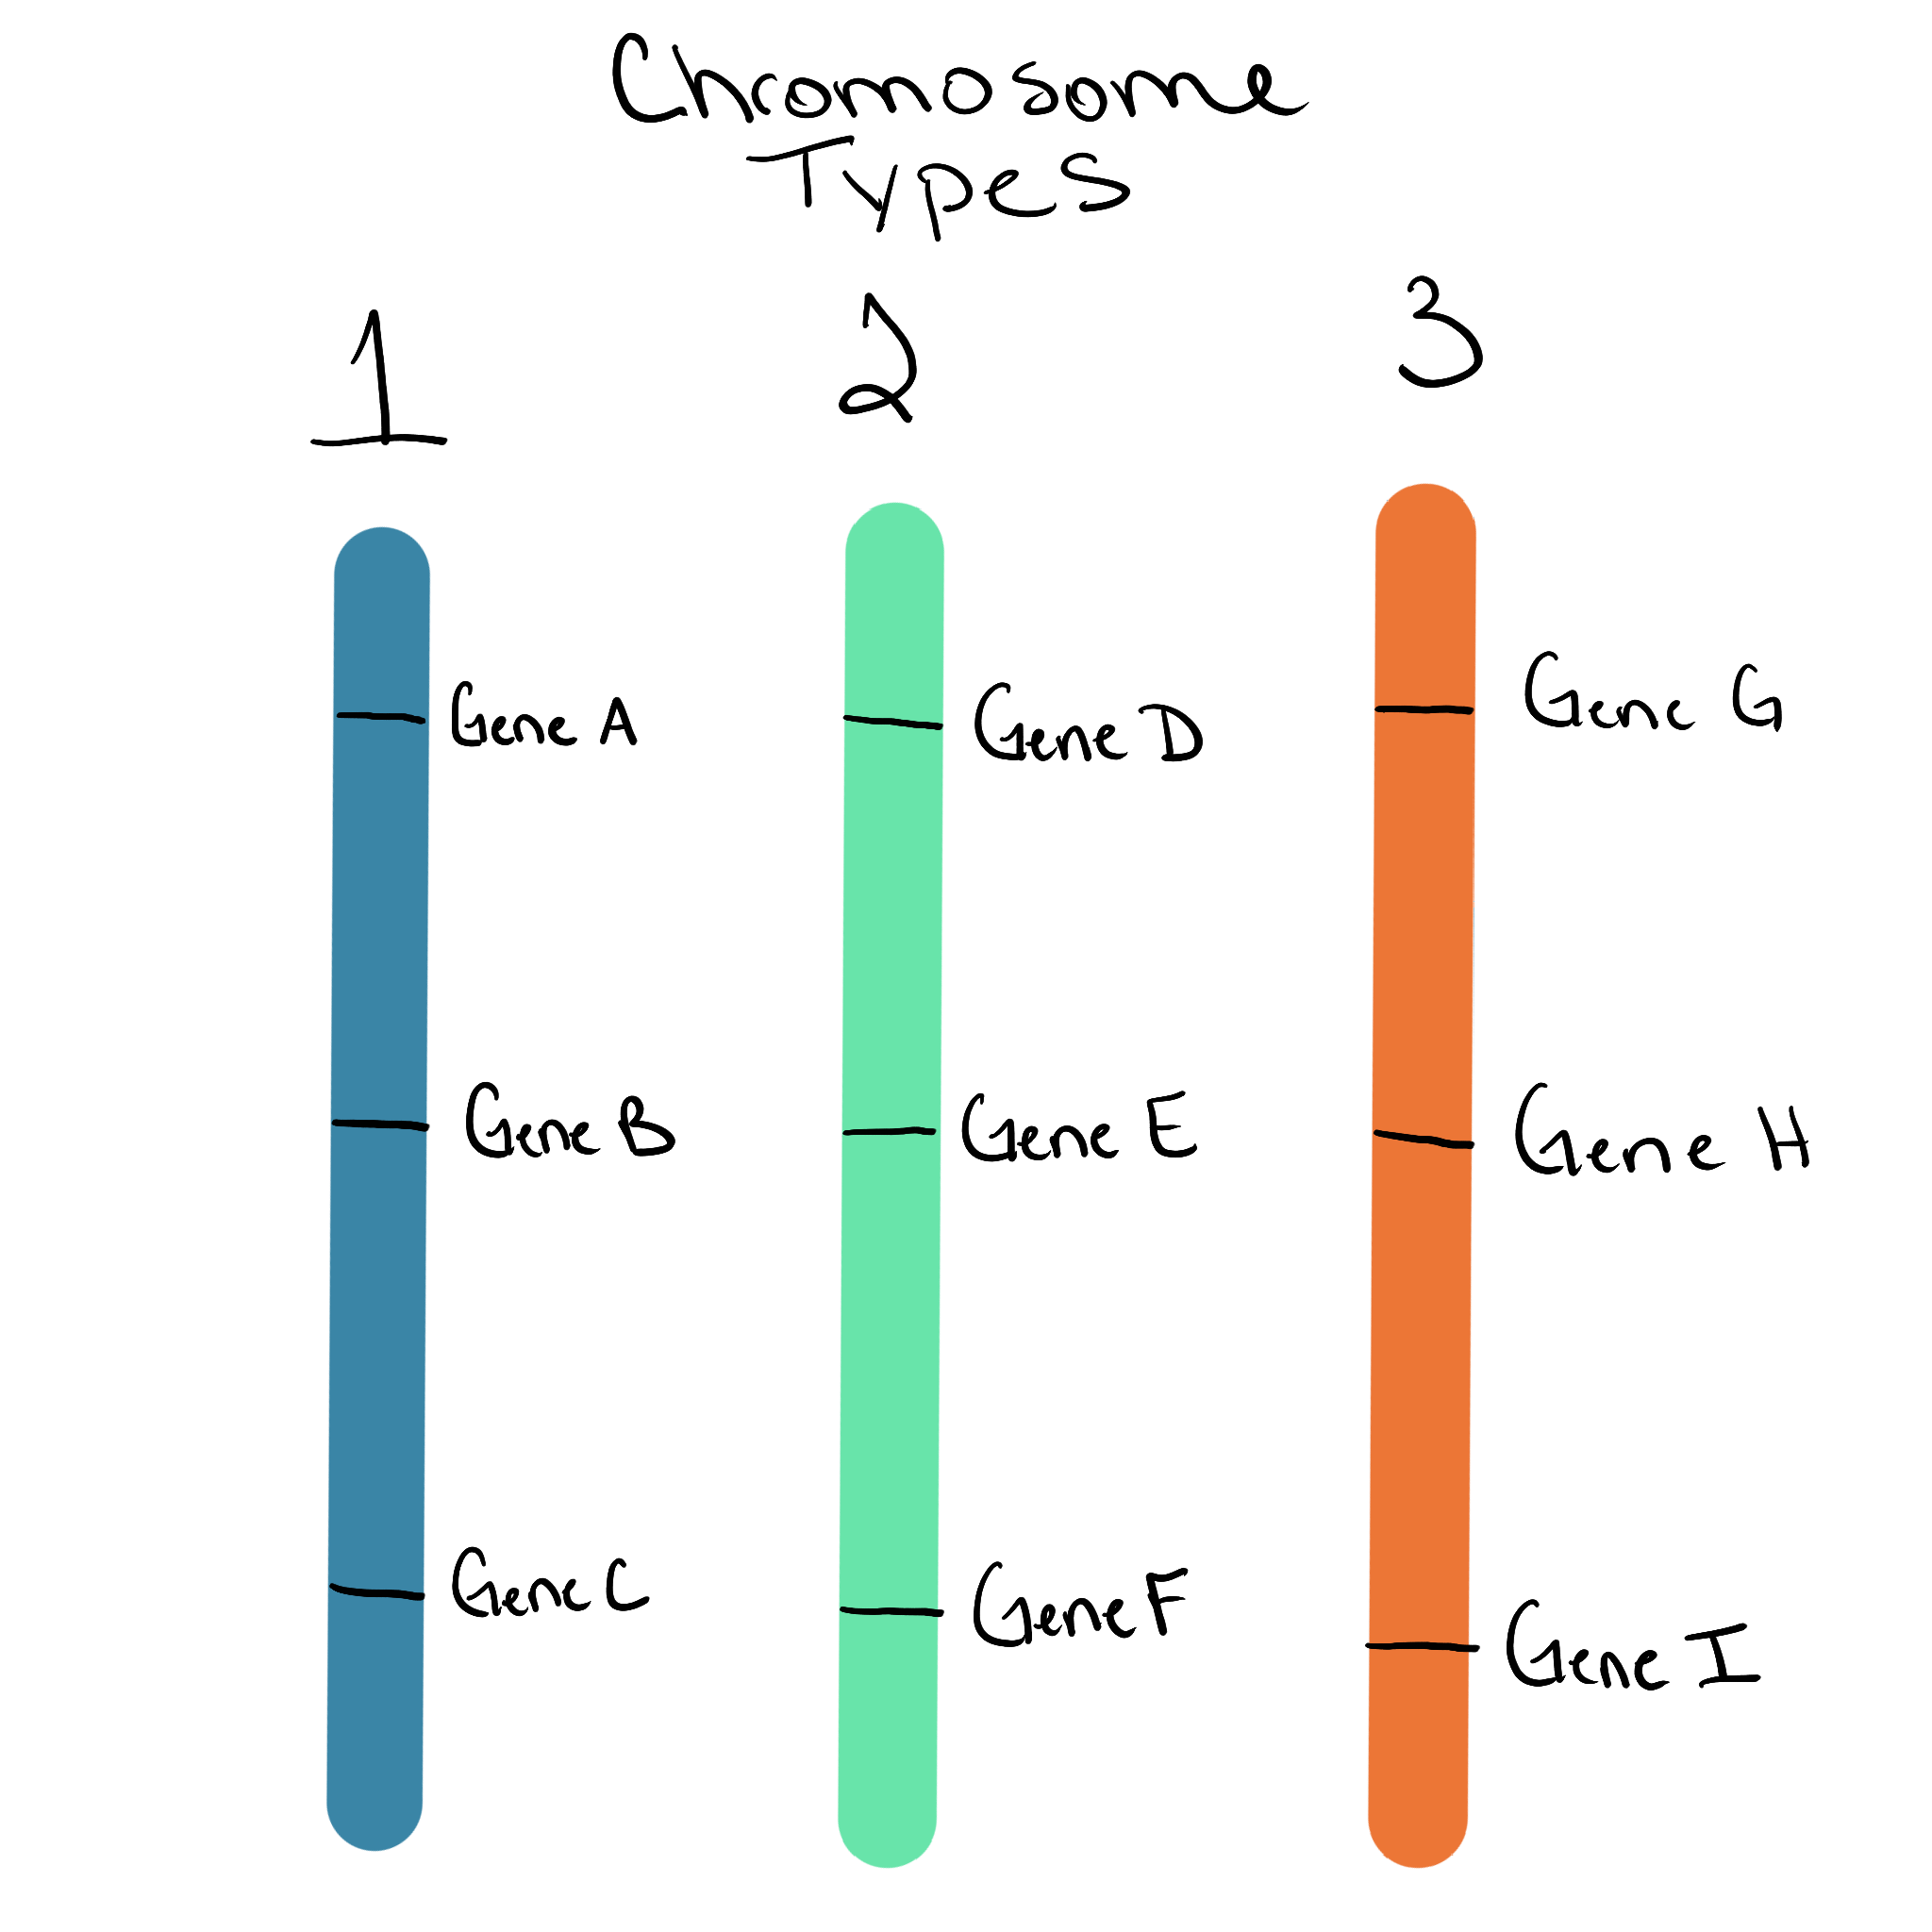
\includegraphics[width=1\linewidth,height=\textheight,keepaspectratio]{../images/chromosome_types.png}
\emph{Figure 2. Different chromosomes contain different genes.}

\begin{tcolorbox}[enhanced jigsaw, colframe=quarto-callout-note-color-frame, leftrule=.75mm, bottomrule=.15mm, opacitybacktitle=0.6, opacityback=0, left=2mm, rightrule=.15mm, coltitle=black, bottomtitle=1mm, titlerule=0mm, toptitle=1mm, breakable, title=\textcolor{quarto-callout-note-color}{\faInfo}\hspace{0.5em}{Important distinction}, colbacktitle=quarto-callout-note-color!10!white, arc=.35mm, toprule=.15mm, colback=white]

Two chromosomes are only considered the ``same type'' if they carry the
\textbf{same genes in the same order}.

\end{tcolorbox}

\begin{center}\rule{0.5\linewidth}{0.5pt}\end{center}

\subsection{Different species have different numbers of chromosome
types}\label{different-species-have-different-numbers-of-chromosome-types}

There is \textbf{no universal chromosome number}.

Examples: - Humans: 23 chromosome types - Dogs: 39 chromosome types -
Fruit flies: 4 chromosome types - Some plants: hundreds

\begin{tcolorbox}[enhanced jigsaw, colframe=quarto-callout-note-color-frame, leftrule=.75mm, bottomrule=.15mm, opacitybacktitle=0.6, opacityback=0, left=2mm, rightrule=.15mm, coltitle=black, bottomtitle=1mm, titlerule=0mm, toptitle=1mm, breakable, title=\textcolor{quarto-callout-note-color}{\faInfo}\hspace{0.5em}{Do not assume}, colbacktitle=quarto-callout-note-color!10!white, arc=.35mm, toprule=.15mm, colback=white]

More chromosomes does \textbf{not} mean ``more complex.''

\end{tcolorbox}

\begin{center}\rule{0.5\linewidth}{0.5pt}\end{center}

\subsection{What are homologous chromosomes
(homologs)?}\label{what-are-homologous-chromosomes-homologs}

In many organisms, chromosomes come in \textbf{sets}.

\textbf{Homologous chromosomes} (or \textbf{homologs}) are the same
chromosome type meaning each chromosome in the set has the same gene
content in the same order.


\includegraphics[width=0.95\linewidth,height=\textheight,keepaspectratio]{../images/chromosomes/homologous_chromosomes.png}
\emph{Figure 4. A homologous pair of chromosomes.}

\begin{center}\rule{0.5\linewidth}{0.5pt}\end{center}

\subsection{Homologs have the same genes, but not necessarily the same
alleles}\label{homologs-have-the-same-genes-but-not-necessarily-the-same-alleles}

This point is \emph{critical}.

\textbf{Homologous chromosomes:} - have the \textbf{same genes} - have
those genes in the \textbf{same locations} - may carry \textbf{different
alleles}

\begin{tcolorbox}[enhanced jigsaw, colframe=quarto-callout-note-color-frame, leftrule=.75mm, bottomrule=.15mm, opacitybacktitle=0.6, opacityback=0, left=2mm, rightrule=.15mm, coltitle=black, bottomtitle=1mm, titlerule=0mm, toptitle=1mm, breakable, title=\textcolor{quarto-callout-note-color}{\faInfo}\hspace{0.5em}{What is an allele?}, colbacktitle=quarto-callout-note-color!10!white, arc=.35mm, toprule=.15mm, colback=white]

Allele - different version of a gene. For example, if a gene codes for
flower color, all alleles of that gene code for flower color but one
allele might code for purple flower color while another codes for white
flower color.

\end{tcolorbox}

In the image below the number subscripts next to the gene name
(e.g.~`A') represent the allele. These homologs carry different alleles
for Gene A and C. They carry the same alleles for Gene B.

\includegraphics[width=1\linewidth,height=\textheight,keepaspectratio]{../images/chromosomes/homologs_diff_alleles.png}
\emph{Figure 5. Homologous chromosomes carry the same genes but may have
different alleles.}

\begin{tcolorbox}[enhanced jigsaw, colframe=quarto-callout-important-color-frame, leftrule=.75mm, bottomrule=.15mm, opacitybacktitle=0.6, opacityback=0, left=2mm, rightrule=.15mm, coltitle=black, bottomtitle=1mm, titlerule=0mm, toptitle=1mm, breakable, title=\textcolor{quarto-callout-important-color}{\faExclamation}\hspace{0.5em}{One sentence to memorize}, colbacktitle=quarto-callout-important-color!10!white, arc=.35mm, toprule=.15mm, colback=white]

\textbf{Homologs = same genes, possibly different alleles.}

\end{tcolorbox}

\begin{center}\rule{0.5\linewidth}{0.5pt}\end{center}

\subsection{Homologs vs different chromosomes (do not mix these
up)}\label{homologs-vs-different-chromosomes-do-not-mix-these-up}

\begin{longtable}[]{@{}lll@{}}
\toprule\noalign{}
Comparison & Homologous chromosomes & Different chromosomes \\
\midrule\noalign{}
\endhead
\bottomrule\noalign{}
\endlastfoot
Gene content & Same genes & Different genes \\
Gene order & Same order & Different \\
Alleles & May differ & Not comparable \\
\end{longtable}

\begin{center}\rule{0.5\linewidth}{0.5pt}\end{center}

\subsection{How many copies of each chromosome are
there?}\label{how-many-copies-of-each-chromosome-are-there}

This depends on the organism and the cell type.

Examples: - \textbf{Diploid cells}: two homologs of each chromosome type
- \textbf{Haploid cells}: one copy of each chromosome type -
\textbf{Polyploid cells}: more than two copies

-\textgreater{} add img of chromosome copy number

\begin{tcolorbox}[enhanced jigsaw, colframe=quarto-callout-note-color-frame, leftrule=.75mm, bottomrule=.15mm, opacitybacktitle=0.6, opacityback=0, left=2mm, rightrule=.15mm, coltitle=black, bottomtitle=1mm, titlerule=0mm, toptitle=1mm, breakable, title=\textcolor{quarto-callout-note-color}{\faInfo}\hspace{0.5em}{Preview}, colbacktitle=quarto-callout-note-color!10!white, arc=.35mm, toprule=.15mm, colback=white]

The number of complete sets of homologs is called \textbf{ploidy} ---
that's next.

\end{tcolorbox}

\begin{center}\rule{0.5\linewidth}{0.5pt}\end{center}

\subsection{Big picture summary}\label{big-picture-summary}

\begin{itemize}
\tightlist
\item
  A \textbf{chromosome} is a single DNA molecule containing many genes
\item
  Different chromosomes carry \textbf{different genes}
\item
  \textbf{Homologous chromosomes} are the same chromosome type carrying
  the same genes but may have different alleles
\item
  Species can differ in:

  \begin{itemize}
  \tightlist
  \item
    number of chromosome types
  \item
    number of copies of those chromosomes
  \end{itemize}
\end{itemize}




\end{document}
